\section{Probabilistic Models of Choice}
\label{in:sec:models}

In this section, we introduce the statistical models and associated methods that will be used or referred to throughout this thesis.
We take a historical perspective: the context in which these models and methods were developed is fascinating.
Although this section only gives a brief overview of the developments, it contains pointers for the reader interested in more comprehensive information.

\subsection{Thurstone's Model}
\label{in:sec:thurstone}

In 1927, Thurstone published an article that is widely regarded as foundational in the field of probabilistic models of comparison outcomes \citep{thurstone1927law}.
He was interested in the problem of measurement in psychology and developed a method that explains the responses of human subjects to comparisons between two stimuli among $N$.
In order to capture the fact that the response to a stimulus can vary, Thurstone suggested modeling the perceived value of a stimulus $i$ during some experiment by means of a \emph{random} variable $x_i \in \mathbf{R}$.
The outcome of the comparison between stimuli $i$ and $j$ is given by comparing a realization of the corresponding two random variables, i.e., by the event $x_i > x_j$.
He further postulated that these random variables follow a jointly Gaussian distribution $\bm{x} \sim \DNorm{\bm{\theta}, \bm{\Sigma}}$.
Denoting by $i \succ j$ the event ``$i$ wins over $j$'',
\begin{align*}
\Prob{i \succ j} = \Prob{x_i > x_j} = \Phi \left( \frac{\theta_i - \theta_j}{\sqrt{\Sigma_{ii} + \Sigma_{jj} - 2\Sigma{ij}}} \right),
\end{align*}
where $\Phi(\cdot)$ is the cumulative density function of the standard normal distribution and the last equality is obtained by noting that $x_i - x_j \sim \DNorm{\theta_i - \theta_j, \Sigma_{ii} + \Sigma_{jj} - 2\Sigma{ij}}$.
Thurstone considered several variants of the model that place successively more restrictive assumptions on the covariance matrix $\bm{\Sigma}$.
The variant that is perhaps most widely-used nowadays is obtained by setting $\bm{\Sigma} = \tfrac{1}{2} \bm{I}$.
In this case,
\begin{align}
\label{in:eq:thu5}
\Prob{i \succ j} = \Phi(\theta_i - \theta_j).
\end{align}
The vector of $N$ parameters $\bm{\theta} = [\theta_1 \ \cdots \ \theta_N]^\Tr \in \mathbf{R}^N$ drives the probabilities of all $\binom{N}{2}$ possible pairwise comparisons.
Intuitively, $\theta_i$ can be interpreted as the \emph{score} of stimulus $i$, and the probability of observing a comparison outcome for $i$ and $j$ that is consistent with the true order increases with the distance $\theta_i - \theta_j$.
Note that as~\eqref{in:eq:thu5} only involves pairwise distances, the parameters $\bm{\theta}$ are identifiable only up to a constant.
In order to resolve this ambiguity, the parameters are often chosen such that $\sum_i \theta_i = 0$.

Perhaps the first application that Thurstone had in mind relates to psychophysics.
Imagine being given two balls and asked the question: ``Which of these two balls is heavier''?
Given a collection of observations of this sort (some of which are possibly inconsistent), model~\eqref{in:eq:thu5} could be used to embed the stimuli on a real-valued scale (compactly summarizing all the data) by means of estimating the parameters $\bm{\theta}$.

\paragraph{Application to Social Values}
Thurstone quickly realized that there was potential beyond psychophysics.
The same year, he published a study in which the method is applied to social values \citep{thurstone1927method}.
This study seeks to understand the seriousness of \num{19} different criminal offenses in the United States, including crimes such as \emph{bootlegging}, \emph{arson}, \emph{seduction} and \emph{homicide}.
Subjects (266 undergraduate students) were instructed to answer a questionnaire containing pairwise comparison questions of the type: ``Which crime is more serious, $i$ or $j$?''
The study perfectly illustrates the advantage of eliciting feedback in the form of comparisons rather than absolute ratings.
Arguably, it would have been very difficult for the subjects to give a numerical score to each crime in a consistent way: in absolute terms, many crimes are extremely serious, and only relative judgments can make nuances appear.

Based on the outcomes of comparisons and using~\eqref{in:eq:thu5}, Thurstone used a least-squares procedure to estimate the parameters $\bm{\theta}$.
This enabled the representation of crimes on a global scale from least to most serious, in a way that reflected the subjects' opinions.
Using the data tabulated in his \citeyear{thurstone1927method} paper, we could replicate\footnote{%
The method used to fit the parameters of the model differs slightly from that of \citet{thurstone1927method}.
However, the differences with the original plot are almost not perceptible.} the analysis he performed.
Figure~\ref{in:fig:crimescale} displays the resulting scale.

\begin{figure}[ht]
\centering
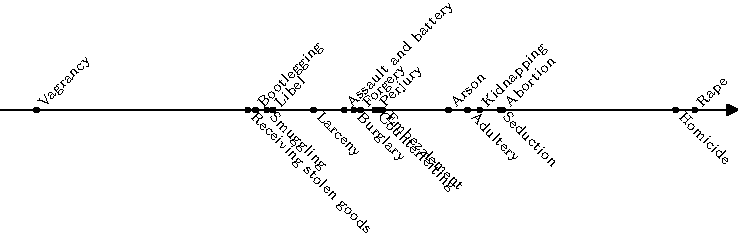
\includegraphics[width=\linewidth]{in-crimescale}
\caption{
Scale of seriousness of offenses (from left to right: least to most serious), using the data in \citet{thurstone1927method}.
Nineteen crimes are embedded on a scale using Thurstone's model, based on 266 students' answers to 171 pairwise comparisons each.
}
\label{in:fig:crimescale}
\end{figure}


\paragraph{A Note on Inference}
The first approaches to learning the parameter vector $\bm{\theta}$ from data relied on least-squares fitting \citep{thurstone1927method, mosteller1951remarks}.
Nowadays, maximum-likelihood estimation is more common.
Indeed, the likelihood~\eqref{in:eq:thu5} is log-concave in $\bm{\theta}$, and standard off-the-shelf convex solvers can be used to find the maximizer.
It is also interesting to note that Thurstone's model lends itself particularly well to approximate Bayesian inference methods \citep{chu2005extensions, chu2005preference}.
An important quantity in Bayesian inference is the \emph{marginal likelihood}, typically of the form
\begin{align*}
\int_{\mathbf{R}^N} \Prob{i \succ j \mid \bm{\theta}} \DNorm{\bm{\theta} \mid \bm{\mu}, \bm{S}} d\bm{\theta}.
\end{align*}
In the case of Thurstone's model, this integral admits a simple closed-form solution. See, e.g., \citet[Section~3.9]{rasmussen2006gaussian}.


\subsection{Bradley--Terry Model}
\label{in:sec:btmodel}

Almost concurrently to Thurstone, Zermelo proposed (in German) a method for ranking chess players based on match outcomes \citep{zermelo1928berechnung}.
He set out to address two problems:
\begin{enuminline}
\item coping with \emph{unbalanced} tournaments, where players play an unequal number of games and against different sets of opponents, and
\item estimating the \emph{relative strength} of players in a way that is predictive of future match outcomes.
\end{enuminline}
%He noted that the system (most widely used the time) based on points awarded to the winner of each match failed to address these.
To this end, he advanced a probabilistic model of game outcomes.
In his model, every player $i \in [N]$ is characterized by a latent strength parameter $\gamma_i \in \mathbf{R}_{>0}$.
The probability of player $i$ winning against player $j$ is a function of their relative strength:
\begin{align}
\label{in:eq:zermelo}
\Prob{i \succ j} = \frac{\gamma_i}{\gamma_i + \gamma_j}.
\end{align}
Note that the parameters $\bm{\gamma}$ are identifiable only up to a multiplicative factor;
for this reason, it is often assumed that $\sum_i \gamma_i = 1$.
Zermelo suggested finding the parameters $\bm{\gamma}$ by maximizing their likelihood given the observed data, an idea that was very advanced at the time.
He formulated a necessary and sufficient condition\footnote{%
The maximum-likelihood estimate exists if and only if there is no way to partition all players into two disjoint non-empty subsets $A, B \subset [N]$, such that there is no player in $A$ that has won a match against a player in $B$.
See also Theorem~\ref{fi:thm:mlboth}.}
for the existence of a unique maximum-likelihood estimate, developed an iterative algorithm\footnote{%
Interestingly, the same algorithm was later rediscovered multiple times in different contexts \citep{bradley1952rank, ford1957solution, dykstra1960rank, hastie1998classification, hunter2004mm, caron2012efficient}.}
to find it and proved the algorithm's convergence.
Overall, his treatment of the model is very thorough and complete; unfortunately it appears to have been largely ignored for about 50 years \citep{david1988method}.
See \citet{glickman2013introductory} for a compelling introduction to Zermelo's paper.
Finally, note that the chess rating system presently in use by the World Chess Federation is directly based on Zermelo's model \citep{elo1978rating}.

\paragraph{Relation to Thurstone's Model}
Over two decades later, \citet{bradley1952rank}, apparently unaware of Zermelo's work, rediscovered the model in the context of the rank analysis of experiments based on pairwise comparisons, linking the model back to the analysis of human opinions.
The connection to Thurstone's model began becoming clear in \citet{bradley1953some}, where Bradley shows that by setting $\theta_i = \log \gamma_i$ for all $i$, the probability~\eqref{in:eq:zermelo} can be rewritten as
\begin{align}
\label{in:eq:bt}
\Prob{i \succ j} = \frac{1}{1 + \exp[-(\theta_i - \theta_j)]}.
\end{align}
Hence, the Bradley--Terry model (as it is commonly referred to) is another instance of a ``generalized linear model'' for pairwise comparisons: the outcome probability depends on the distance $\theta_i - \theta_j$ between the two parameters corresponding to the score of the alternatives.
\citet{yellot1977relationship} further expanded the connection, by showing that $\Prob{i \succ j}$ in~\eqref{in:eq:bt} can be rewritten as $\Prob{x_i > x_j}$ for independent random variables $\{x_k : k \in [N]\}$ such that $x_k \sim \DGumbel{\theta_k, 1}$, that is, $\Prob{x_k \le y} = \exp\{-\exp[-(y - \theta_k)]\}$.
Outcomes can therefore also be thought of as the comparison of the realizations of two random variables centered around the alternatives' scores, similarly to Thurstone's model, which gave rise to a \emph{random utility} interpretation.
Finally, \citet{stern1992all} showed that both Thurstone's and the Bradley--Terry model can be unified under a more general model using the gamma distribution.
In practice, both models give quantitatively similar results in most cases~\citep{tsukida2011how}.
Figure~\ref{in:fig:sigmoids} illustrates the probabilities~\eqref{in:eq:thu5} and~\eqref{in:eq:bt} as a function of $\theta_i - \theta_j$.

\begin{figure}
\centering
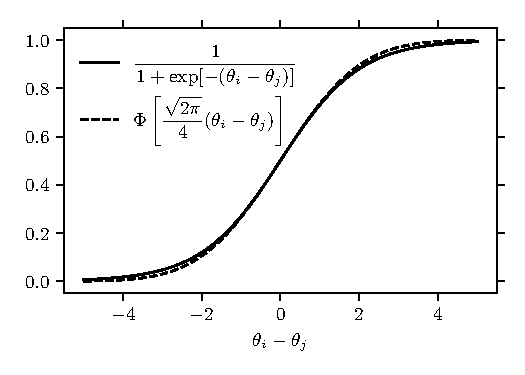
\includegraphics{in-sigmoids}
\caption{
Comparison of the Bradley--Terry model and a rescaled version of Thurstone's model.
The scaling constant is chosen such that the slope at the origin matches.
}
\label{in:fig:sigmoids}
\end{figure}


\subsection{Luce's Choice Axiom}
\label{in:sec:choice}

The two models discussed above are limited to comparisons between \emph{pairs} of items.
How to generalize these models to \emph{multiway} comparisons?
Given a set of alternatives $\mathcal{A} \subseteq [N]$ and an item $i \in \mathcal{A}$, denote by $i \succeq \mathcal{A}$ the event ``$i$ is chosen among alternatives $\mathcal{A}$''.
A natural way to extend the Bradley--Terry model~\eqref{in:eq:zermelo} to choices among arbitrarily many alternatives is as follows:
\begin{align}
\label{in:eq:luce}
\Prob{i \succeq \mathcal{A}} = \frac{\gamma_i}{\sum_{j \in \mathcal{A}} \gamma_j}.
\end{align}
Simply put, the probability of a choice is always proportional to the strength $\gamma_i$ of the item $i$, no matter what the set of alternatives is.
This choice model is due to \citet{luce1959individual}, who showed that it is closely related to the following property.

\begin{definition}[independence of irrelevant alternatives]
A probabilistic choice model is said to satisfy the \emph{independence from irrelevant alternatives} (IIA) property if for any $\mathcal{A} \subseteq [N]$ and any $i, j \in \mathcal{A}$,
\begin{align*}
\frac{\Prob{j \succeq \mathcal{A}}}{\Prob{i \succeq \mathcal{A}}}
     = \frac{\Prob{j \succ i}}{\Prob{i \succ j}}.
\end{align*}
\end{definition}

The IIA property is essentially equivalent\footnote{%
\citet{luce1959individual} introduces the IIA property as a consequence of the choice axiom, which is slightly more general: its formulation permits $\Prob{i \succeq \mathcal{A}} = 0$, a technicality that we will not consider in this thesis.}
to Luce's \emph{choice axiom} \citeyearpar[p. 6]{luce1959individual}, and in this thesis we will refer to these two concepts interchangeably.
Luce's fundamental contribution was to show that the IIA property enables an axiomatic characterization of the choice probabilities.

\begin{proposition}
A choice model satisfies the IIA property if and only if there exists a vector $\bm{\gamma} \in \mathbf{R}_{>0}$ such that the choice probabilities are given by~\eqref{in:eq:luce}.
\end{proposition}

\begin{proof}
It is trivial to verify that choice probabilities given by~\eqref{in:eq:luce} satisfy IIA for any $\bm{\gamma}$.
We will now show that the IIA property actually implies the existence of such a parametric representation of choice probabilities.
Let $z \in [N]$ be an arbitrary alternative, and let
\begin{align*}
\gamma_i =
\begin{cases}
\Prob{i \succ z} / \Prob{z \succ i} & \text{if $i \ne z$,} \\
1                                   & \text{otherwise.} \\
\end{cases}
\end{align*}
Let $\mathcal{A} \subseteq [N]$ be any (non-empty) set of alternatives, and let $\mathcal{B} = \mathcal{A} \cup \{ z \}$.
By IIA,
\begin{align*}
&\Prob{i \succeq \mathcal{B}} = \gamma_i \Prob{z \succeq \mathcal{B}}
    \qquad \forall i \in \mathcal{B} \\
&\quad \implies
    \frac{\Prob{j \succeq \mathcal{B}}}{\Prob{i \succeq \mathcal{B}}}
    = \frac{\gamma_j}{\gamma_i}
    = \frac{\Prob{j \succ i}}{\Prob{i \succ j}}
    = \frac{\Prob{j \succeq \mathcal{A}}}{\Prob{i \succeq \mathcal{A}}}
    \qquad \forall i, j \in \mathcal{A} \\
&\quad \implies \Prob{j \succeq \mathcal{A}} = \frac{\gamma_j}{\gamma_i} \Prob{i \succeq \mathcal{A}}
    \qquad \forall i, j \in \mathcal{A}.
\end{align*}
Furthermore, as $\sum_{j \in \mathcal{A}} \Prob{j \succeq \mathcal{A}} = 1$, we have, for all $i \in \mathcal{A}$,
\begin{align*}
1 = \sum_{j \in \mathcal{A}} \frac{\gamma_j}{\gamma_i} \Prob{i \succeq \mathcal{A}}
    \implies \Prob{i \succeq \mathcal{A}} = \frac{\gamma_i}{\sum_{j \in \mathcal{A}} \gamma_j},
\end{align*}
which concludes the proof.
\end{proof}

Independence of irrelevant alternatives is a powerful property, as it leads to a choice model that represents \emph{combinatorially} many choice probabilities by using only $N$ parameters.
This makes tractable the problem of learning the choice probabilities from a possibly small number of observations, but it inevitably restricts the expressivity of the model.
In cases where some alternatives are very similar, IIA can turn out to be unrealistic, as shown by \citet{debreu1960review} in a simple example.
In the context of modern applications with a large number of items, which is the focus of this thesis, we believe that this trade-off is acceptable (and perhaps even necessary).

\paragraph{Extension to Rankings}
Numerous extensions of Luce's choice model have been proposed in the literature, enabling the analysis of observations beyond those of the type ``one out of $K$''.
Perhaps one of the most widely-used extensions relates to ranking.
Letting $i(r)$ be the item of rank $r$, \citet{plackett1975analysis} suggested modeling the probability of a ranking on $K \le N$ items as
\begin{align*}
\Prob{i(1) \succ i(2) \succ \cdots \succ i(K)} = \prod_{r = 1}^{K - 1} \frac{\gamma_{i(r)}}{\sum_{s = r}^K \gamma_{i(s)}},
\end{align*}
for some $\bm{\gamma} \in \mathbf{R}_{>0}$.
This can be seen as $K-1$ independent choices made using Luce's model, iteratively, over the remaining alternatives.
Therefore, this model is referred to as the \emph{Plackett--Luce} model.

\paragraph{Random Utility Models}
Finally, we note that all the models discussed so far can be analyzed and generalized in the framework of \emph{random utility models} \citep{train2009discrete}.
This enables, for example, an extension of Thurstone's model to multiway comparisons, in a similar way to Luce's extension of the Bradley--Terry model.
In this framework, the choice probabilities are defined by the probability of certain orderings of a collection of random variables (representing the utility of the alternatives).

% modern advances (I think this is not necessary here):
% - inference: ML (hunter), Bayesian (Chu / Ghahramani, caron/doucet), spectral-based.
% - guarantees: Negahban, Hajek, Vojnovic
